\documentclass[tikz,border=6pt]{standalone}
% Shared visual language for the original benchmark atlas.
\usepackage[T1]{fontenc}
\usepackage{lmodern}
\usepackage{amsmath,amssymb}
\usetikzlibrary{arrows.meta,calc,positioning,shapes.geometric,patterns,decorations.pathmorphing,backgrounds,fit}
\definecolor{ink}{HTML}{173948}
\definecolor{flow}{HTML}{167D9A}
\definecolor{control}{HTML}{A65217}
\definecolor{measure}{HTML}{70518A}
\definecolor{pale}{HTML}{EAF2F5}
\definecolor{muted}{HTML}{526571}
\definecolor{utility}{HTML}{2E8665}
\tikzset{
  every node/.style={font=\sffamily\small,text=ink},
  equipment/.style={draw=ink,line width=1pt,fill=pale,rounded corners=2pt},
  process/.style={draw=flow,line width=1.2pt,-{Latex[length=2.5mm]}},
  signal/.style={draw=control,line width=.8pt,dashed,-{Latex[length=2mm]}},
  util/.style={draw=utility,line width=1pt,-{Latex[length=2.2mm]}},
  dimension/.style={draw=muted,line width=.6pt,{Latex[length=1.7mm]}-{Latex[length=1.7mm]}},
  labelbox/.style={fill=white,inner sep=2pt,font=\sffamily\footnotesize,align=center},
  annotation/.style={font=\sffamily\footnotesize,text=muted,align=left},
  panel/.style={draw=ink!20,fill=ink!2,rounded corners=3pt,inner sep=6pt},
  instrument/.style={circle,draw=measure,fill=white,line width=.8pt,minimum size=8mm,inner sep=1pt,font=\sffamily\scriptsize,align=center},
  port/.style={circle,fill=flow,inner sep=1.6pt},
  box/.style={equipment,minimum width=3cm,minimum height=1cm,align=center},
}
\newcommand{\atlasheader}[3]{%
  \node[anchor=north west,font=\sffamily\bfseries\LARGE] at (0,0) {#1};%
  \node[anchor=north west,font=\sffamily\small,text=muted] at (0,-.75) {Paper section #2: \textit{#3}};%
  \draw[ink!25,line width=.7pt] (0,-1.25)--(26,-1.25);%
}
\newcommand{\atlasfooter}[1]{%
  \draw[ink!25,line width=.5pt] (0,-15.8)--(26,-15.8);%
  \node[anchor=north west,annotation,text width=25.8cm] at (0,-16) {#1\\Original explanatory drawing. Source: Kroll \& Schulte (2014), DOI: 10.1016/j.asoc.2014.08.034. Model variants are identified in the accompanying case sheet.};%
}

\usetikzlibrary{shadings,shadows}
% Industrial presentation of the reviewed SI hydrostatic transmission.
% The surrounding workshop, casing details, fasteners and lighting are
% illustrative ONLY. They introduce no new states, sensors or flow paths.
% Keep the benchmark circuit topology and calibrated/noncalibrated meaning.
% TikZ.net drawing references (not copied artwork):
% https://tikz.net/mechanical-systems/ -- precise mechanical links and nodes.
% https://tikz.net/fluid_dynamics_pressure/ -- metal/fluid gradations and flow arrows.
% https://tikz.net/fluid_dynamics_barometer/ -- layered tubular paths.
\definecolor{hydWall}{HTML}{F3F1E9}
\definecolor{hydSage}{HTML}{DDE8E0}
\definecolor{hydSteel}{HTML}{677F86}
\definecolor{hydSteelMid}{HTML}{BBCBCD}
\definecolor{hydSteelHi}{HTML}{F9F9F3}
\definecolor{hydGraphite}{HTML}{304A54}
\definecolor{hydRubber}{HTML}{344146}
\definecolor{hydTeal}{HTML}{458FA5}
\definecolor{hydTealHi}{HTML}{B5E0E5}
\definecolor{hydBronze}{HTML}{B78950}
\definecolor{hydSand}{HTML}{F7F1E6}
\definecolor{hydSky}{HTML}{D7E8ED}
\newcommand{\hydshaft}[1]{%
  \draw[hydGraphite,line width=3.4pt,line cap=butt] #1;
  \draw[hydSteelMid,line width=2.5pt,line cap=butt] #1;
  \draw[hydSteelHi,line width=.6pt,line cap=butt,opacity=.92] #1;
}
% Coaxial metal casing/blue hydraulic core; arrows remain directional.
\newcommand{\hydpipe}[1]{%
  \draw[hydGraphite!85,line width=4.0pt,line join=round] #1;
  \draw[hydSteelMid,line width=3.0pt,line join=round] #1;
  \draw[flow,line width=1.9pt,line join=round,-{Latex[length=2.6mm]}] #1;
}
% Physically descriptive but intentionally nonstandard housing illustration.
\newcommand{\hydmachine}[2]{%
  \shade[draw=hydGraphite,line width=1.1pt,inner color=hydSteelHi,
    outer color=hydSteelMid] (#1,#2) circle (1.30);
  \shade[draw=hydSteel!85,line width=.55pt,inner color=hydSteelHi,
    outer color=hydTeal!38!hydSteelMid] (#1,#2) circle (1.14);
  \draw[hydGraphite!65,line width=.65pt] (#1,#2) circle (1.18);
  \foreach \a in {45,135,225,315}{%
    \shade[draw=hydGraphite,line width=.28pt,top color=hydSteelHi,
      bottom color=hydSteel] ($(#1,#2)+(\a:1.23)$) circle (.075);
    \fill[hydGraphite] ($(#1,#2)+(\a:1.23)$) circle (.022);
  }
  \draw[white,opacity=.74,line width=1.0pt]
    ($(#1,#2)+(145:1.04)$) arc[start angle=145,end angle=225,radius=1.04];
}
\tikzset{
  hydPanelA/.style={panel,fill=hydSky!62!white,draw=hydSteel!32},
  hydPanelB/.style={panel,fill=hydSage!45!white,draw=hydSteel!32},
  hydPanelC/.style={panel,fill=hydSand!90!white,draw=hydSteel!32}
}

\begin{document}
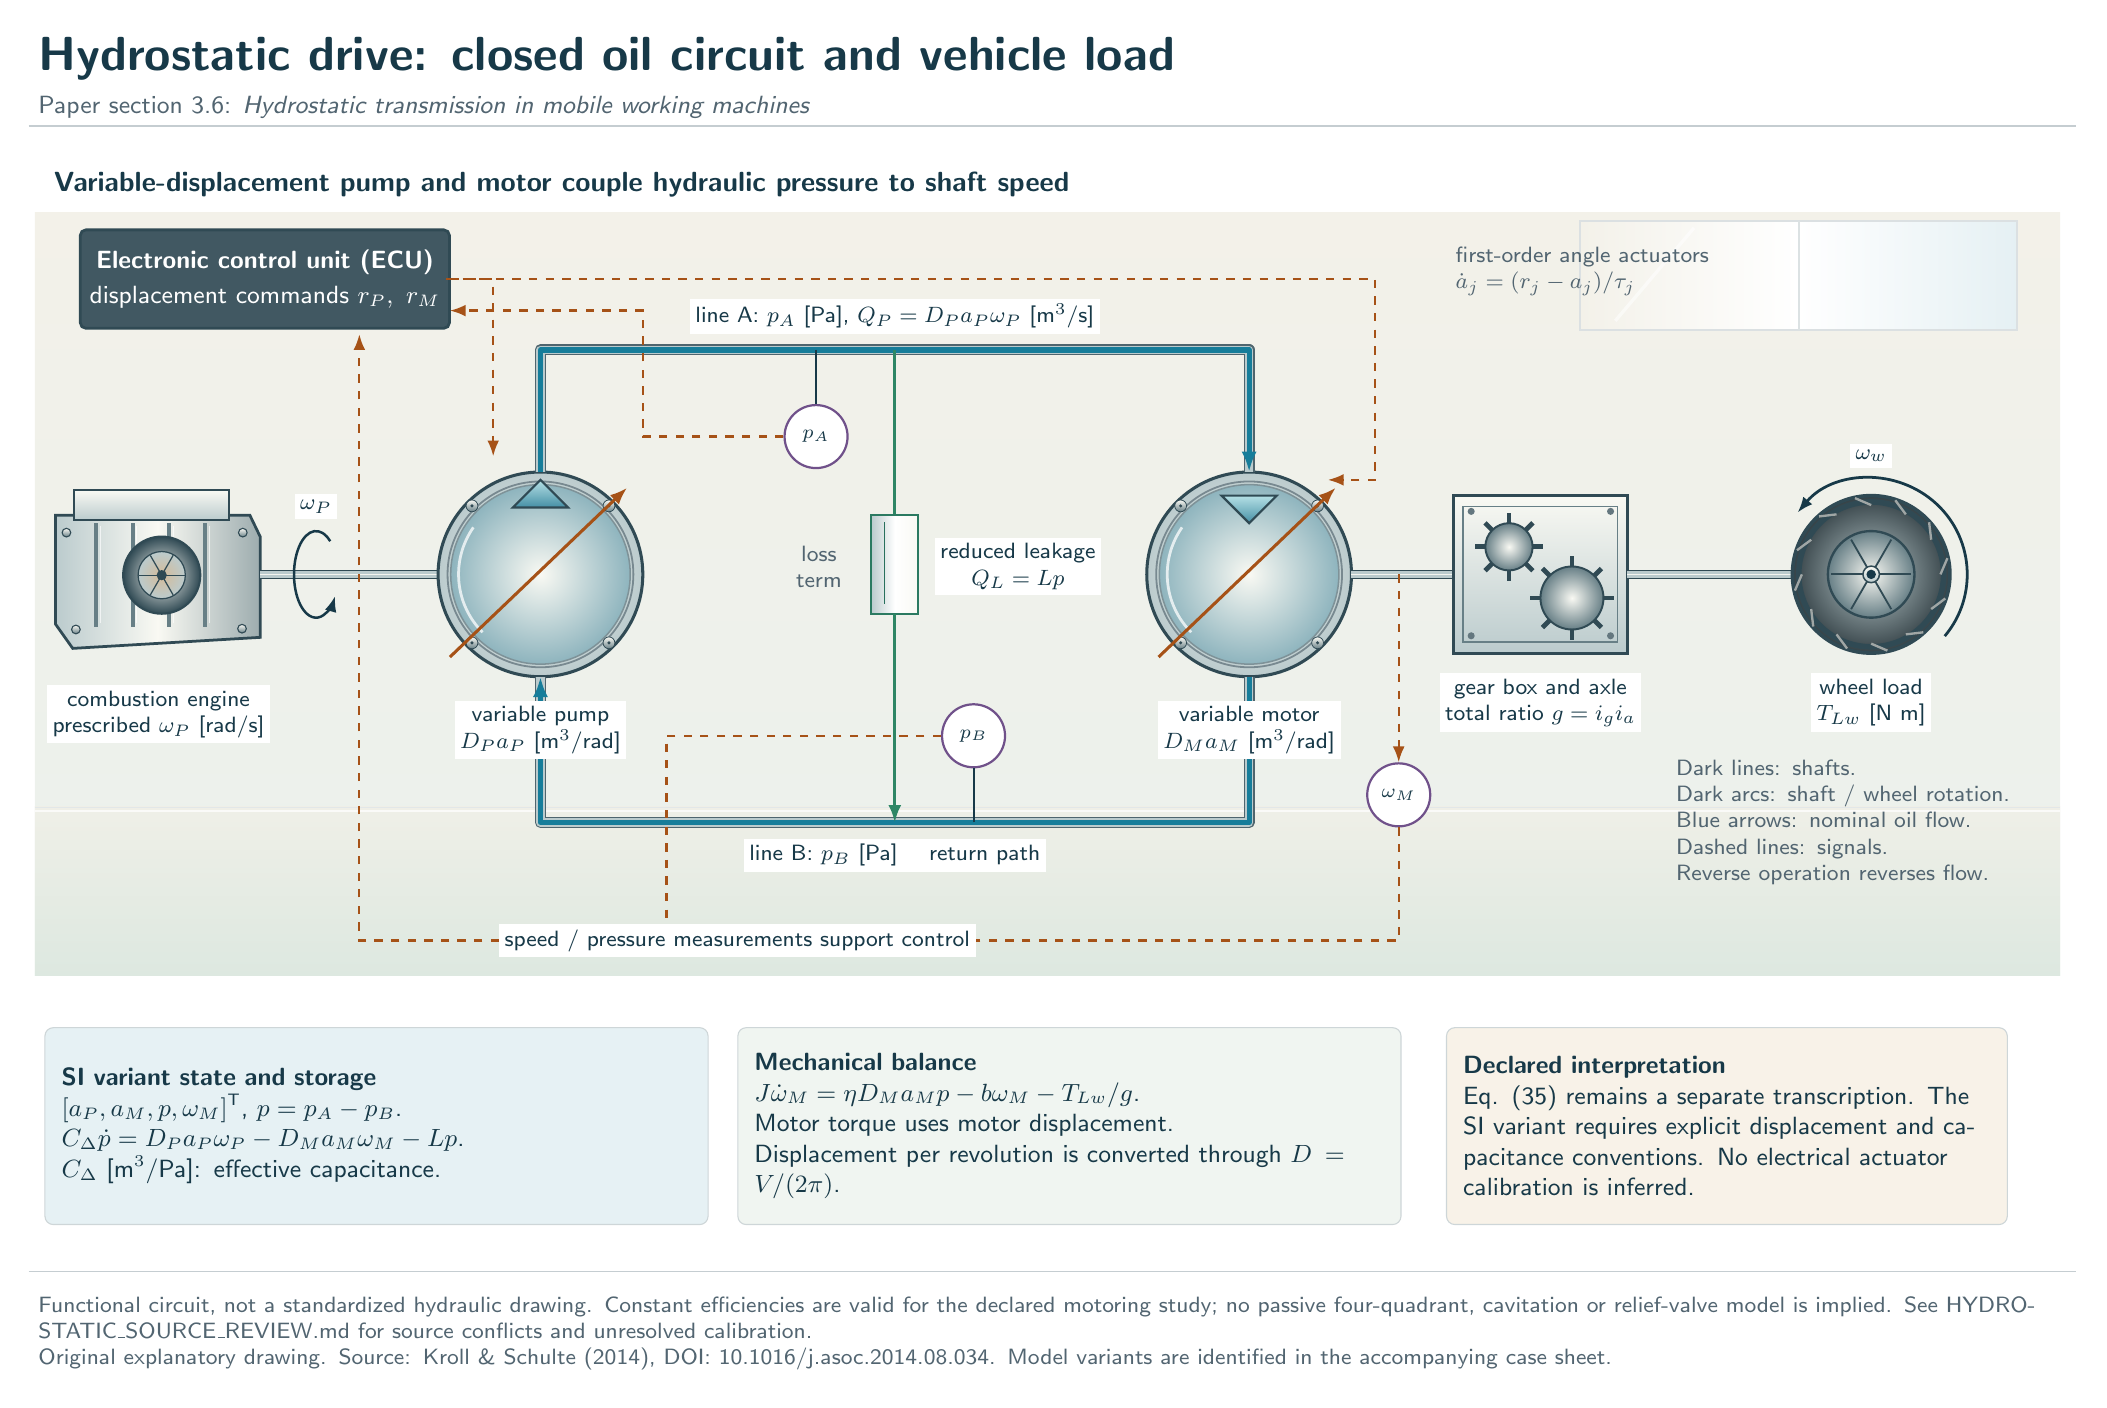
\begin{tikzpicture}[x=1cm,y=1cm]
\atlasheader{Hydrostatic drive: closed oil circuit and vehicle load}{3.6}{Hydrostatic transmission in mobile working machines}
\node[anchor=west,font=\sffamily\bfseries] at (.2,-2) {Variable-displacement pump and motor couple hydraulic pressure to shaft speed};
% Restrained workshop atmosphere: wall, overhead daylight and sage service
% surface. These backgrounds are not modeled process equipment.
\begin{scope}[on background layer]
  \shade[top color=hydWall,bottom color=hydSage!60!white]
    (.08,-2.35) rectangle (25.80,-12.04);
  \shade[top color=hydSage!18!hydWall,bottom color=hydSage]
    (.08,-9.90) rectangle (25.80,-12.04);
  \draw[hydSteel!19,line width=.65pt] (.08,-9.91)--(25.80,-9.91);
  \draw[white,opacity=.75,line width=.65pt] (.08,-9.96)--(25.80,-9.96);
  \shade[left color=hydWall,right color=hydSky!65!white,middle color=white]
    (19.7,-2.46) rectangle (25.25,-3.85);
  \draw[hydSteel!24,line width=.6pt]
    (19.7,-2.46) rectangle (25.25,-3.85);
  \draw[white,opacity=.55,line width=1.2pt]
    (20.15,-3.73)--(21.15,-2.55);
  \draw[hydSteel!23,line width=.6pt] (22.48,-2.46)--(22.48,-3.85);
\end{scope}

% Prime mover: a shaded industrial engine block, not a literal cutaway.
\shade[draw=hydGraphite,line width=1pt,left color=hydSteelMid,
  right color=hydSteel!63!hydSteelHi,middle color=hydSteelHi]
  (.34,-6.20)--(2.81,-6.20)--(2.94,-6.47)--(2.94,-7.75)
  --(.56,-7.89)--(.34,-7.58)--cycle;
\shade[draw=hydGraphite,line width=.8pt,top color=hydSteelHi,
  bottom color=hydSteelMid] (.58,-5.88) rectangle (2.54,-6.26);
\foreach \x in {.86,1.32,1.78,2.24}{
  \draw[hydSteel,line width=1.4pt] (\x,-6.30)--(\x,-7.62);
  \draw[white,opacity=.65,line width=.35pt] (\x+.055,-6.34)--(\x+.055,-7.57);
}
\shade[draw=hydGraphite,line width=.75pt,inner color=hydSteelHi,
  outer color=hydGraphite] (1.69,-6.96) circle (.49);
\shade[draw=hydGraphite,line width=.45pt,inner color=hydBronze!55!hydSteelHi,
  outer color=hydSteelMid] (1.69,-6.96) circle (.30);
\foreach \a in {0,60,...,300}{
  \draw[hydGraphite,line width=.45pt] (1.69,-6.96)--($(1.69,-6.96)+(\a:.29)$);
}
\fill[hydGraphite] (1.69,-6.96) circle (.065);
\foreach \x/\y in {.48/-6.42,2.72/-6.42,.60/-7.65,2.71/-7.64}{
  \shade[draw=hydGraphite,top color=hydSteelHi,bottom color=hydSteel]
    (\x,\y) circle (.055);
}
\node[labelbox,anchor=north] at (1.65,-8.35)
  {combustion engine\\prescribed $\omega_P$ [rad/s]};
\hydshaft{(2.94,-6.95)--(5.20,-6.95)}
% Local shaft coordinates keep the rotation marker centered on the shaft.
\begin{scope}[shift={(3.65,-6.95)}]
\draw[ink,line width=.9pt,-{Latex[length=2mm]}] (50:.28 and .55)
 arc[start angle=50,end angle=330,x radius=.28,y radius=.55];
\end{scope}
\node[labelbox,anchor=south] at (3.65,-6.25) {$\omega_P$};
% Pump and motor: coaxial metal housings; arrows retain the same
% displacement sign and energy-transfer convention as the approved source.
\hydmachine{6.5}{-6.95}
\shade[draw=hydGraphite,line width=.8pt,top color=hydTealHi,
  bottom color=hydTeal] (6.15,-6.10)--(6.85,-6.10)--(6.5,-5.75)--cycle;
\draw[control,-{Latex[length=2.2mm]},line width=1.1pt]
  (5.35,-8)--(7.6,-5.85);
\hydmachine{15.5}{-6.95}
\shade[draw=hydGraphite,line width=.8pt,top color=hydTealHi,
  bottom color=hydTeal] (15.15,-5.95)--(15.85,-5.95)--(15.5,-6.30)--cycle;
\draw[control,-{Latex[length=2.2mm]},line width=1.1pt]
  (14.35,-8)--(16.6,-5.85);
% Closed hydraulic loop and measured line pressures.
\hydpipe{(6.5,-5.65)--(6.5,-4.1)--(15.5,-4.1)--(15.5,-5.65)}
\hydpipe{(15.5,-8.25)--(15.5,-10.1)--(6.5,-10.1)--(6.5,-8.25)}
\node[labelbox,anchor=south] at (11,-3.9) {line A: $p_A$ [Pa], $Q_P=D_Pa_P\omega_P$ [m$^3$/s]};
\node[labelbox,anchor=north] at (11,-10.3) {line B: $p_B$ [Pa] \quad return path};
\node[labelbox,anchor=north] at (6.5,-8.55) {variable pump\\$D_P a_P$ [m$^3$/rad]};
\node[labelbox,anchor=north] at (15.5,-8.55) {variable motor\\$D_M a_M$ [m$^3$/rad]};
\node[instrument] (pa) at (10,-5.2) {$p_A$};
\node[instrument] (pb) at (12,-9) {$p_B$};
\draw[ink,line width=.7pt] (10,-4.1)--(pa.north) (12,-10.1)--(pb.south);
% Internal leakage is an explicit reduced loss, not a relief valve.
\draw[utility,line width=1.0pt] (11,-4.1)--(11,-6.2);
\shade[draw=utility!85!ink,line width=.7pt,left color=hydSteelMid,
  right color=hydSteelHi,middle color=white] (10.7,-6.2) rectangle (11.3,-7.45);
\draw[utility!72!ink,line width=.5pt] (10.87,-6.29)--(10.87,-7.32);
\draw[util] (11,-7.45)--(11,-10.1);
\node[labelbox,anchor=west] at (11.5,-6.85) {reduced leakage\\$Q_L=Lp$};
\node[annotation,anchor=east,align=center] at (10.45,-6.85) {loss\\term};
% Motor shaft, machined gearbox and wheel. Illustrated metal highlights
% describe surfaces only, without altering the drive reduction or load.
\hydshaft{(16.8,-6.95)--(18.1,-6.95)}
\shade[draw=hydGraphite,line width=1.1pt,top color=hydSteelHi,
  bottom color=hydSteelMid] (18.1,-5.95) rectangle (20.3,-7.95);
\draw[hydSteel,line width=.6pt] (18.22,-6.09) rectangle (20.18,-7.81);
\foreach \a in {0,45,...,315}{
  \draw[hydGraphite,line width=1.7pt] ($(18.8,-6.6)+(\a:.3)$)--($(18.8,-6.6)+(\a:.43)$);
  \draw[hydGraphite,line width=1.7pt] ($(19.6,-7.25)+(\a:.4)$)--($(19.6,-7.25)+(\a:.53)$);
}
\shade[draw=hydGraphite,line width=.7pt,inner color=hydSteelHi,outer color=hydSteel]
  (18.8,-6.6) circle (.30);
\shade[draw=hydGraphite,line width=.7pt,inner color=hydSteelHi,outer color=hydSteel]
  (19.6,-7.25) circle (.40);
\foreach \x/\y in {18.32/-6.15,20.09/-6.15,18.32/-7.73,20.09/-7.73}{
  \fill[hydGraphite!75] (\x,\y) circle (.045);
}
\hydshaft{(20.3,-6.95)--(22.4,-6.95)}
\shade[draw=hydGraphite,line width=1.3pt,inner color=hydSteelMid,
  outer color=hydRubber] (23.4,-6.95) circle (1.00);
\draw[hydGraphite,line width=2pt] (23.4,-6.95) circle (.92);
\foreach \a in {0,30,...,330}{
  \draw[hydSteelHi!55!hydRubber,line width=.85pt]
    ($(23.4,-6.95)+(\a:.88)$)--($(23.4,-6.95)+(\a+12:.99)$);
}
\shade[draw=hydGraphite,line width=.85pt,inner color=hydSteelHi,
  outer color=hydSteel] (23.4,-6.95) circle (.55);
\foreach \a in {0,60,...,300}{
  \draw[hydGraphite,line width=.65pt]
    (23.4,-6.95)--($(23.4,-6.95)+(\a:.51)$);
}
\shade[draw=hydGraphite,line width=.55pt,top color=hydSteelHi,
  bottom color=hydSteelMid] (23.4,-6.95) circle (.105);
\node[labelbox,anchor=north] at (19.2,-8.2) {gear box and axle\\total ratio $g=i_gi_a$};
\node[labelbox,anchor=north] at (23.4,-8.2) {wheel load\\$T_{Lw}$ [N m]};
% Rotation is concentric with the wheel, not a displaced material-flow arc.
\fill[ink] (23.4,-6.95) circle (.06);
\begin{scope}[shift={(23.4,-6.95)}]
\draw[ink,line width=1pt,-{Latex[length=2mm]}] (-40:1.22)
 arc[start angle=-40,end angle=140,radius=1.22];
\end{scope}
\node[labelbox,anchor=south] at (23.4,-5.6) {$\omega_w$};
\node[instrument] (speed) at (17.4,-9.75) {$\omega_M$};
\draw[signal] (17.4,-6.95)--(speed.north);
% Displacement control and feedback.
\node[box,draw=hydGraphite,fill=hydGraphite!92,rounded corners=2pt,
  text=white,minimum width=4.6cm,minimum height=1.25cm] (ecu)
  at (3,-3.2) {\textbf{Electronic control unit (ECU)}\\[2pt]
    \color{white!89}displacement commands $r_P,\ r_M$};
\draw[signal] (ecu.east)--(5.9,-3.2)--(5.9,-5.45);
\draw[signal] (5.3,-3.2)--(17.1,-3.2)--(17.1,-5.75)--(16.5,-5.75);
\node[annotation,anchor=west] at (18,-3.1) {first-order angle actuators\\$\dot a_j=(r_j-a_j)/\tau_j$};
\draw[signal] (speed.south)--(17.4,-11.6)--(4.2,-11.6)--(4.2,-3.9);
\draw[signal] (pa.west)--(7.8,-5.2)--(7.8,-3.6)--(5.35,-3.6);
\draw[signal] (pb.west)--(8.1,-9)--(8.1,-11.6);
\node[labelbox] at (9,-11.6) {speed / pressure measurements support control};
\node[annotation,anchor=west,text width=4.6cm] at (20.8,-10.1) {Dark lines: shafts.\\Dark arcs: shaft / wheel rotation.\\Blue arrows: nominal oil flow.\\Dashed lines: signals.\\Reverse operation reverses flow.};
\node[hydPanelA,anchor=north west,text width=8cm,minimum height=2.5cm,align=left] at (.2,-12.7) {\textbf{SI variant state and storage}\\$[a_P,a_M,p,\omega_M]^{\mathsf T}$, $p=p_A-p_B$.\\$C_\Delta\dot p=D_Pa_P\omega_P-D_Ma_M\omega_M-Lp$.\\$C_\Delta$ [m$^3$/Pa]: effective capacitance.};
\node[hydPanelB,anchor=north west,text width=8cm,minimum height=2.5cm,align=left] at (9,-12.7) {\textbf{Mechanical balance}\\$J\dot\omega_M=\eta D_Ma_Mp-b\omega_M-T_{Lw}/g$.\\Motor torque uses motor displacement.\\Displacement per revolution is converted through $D=V/(2\pi)$.};
\node[hydPanelC,anchor=north west,text width=6.7cm,minimum height=2.5cm,align=left] at (18,-12.7) {\textbf{Declared interpretation}\\Eq. (35) remains a separate transcription. The SI variant requires explicit displacement and capacitance conventions. No electrical actuator calibration is inferred.};
\atlasfooter{Functional circuit, not a standardized hydraulic drawing. Constant efficiencies are valid for the declared motoring study; no passive four-quadrant, cavitation or relief-valve model is implied. See HYDROSTATIC\_SOURCE\_REVIEW.md for source conflicts and unresolved calibration.}
\end{tikzpicture}
\end{document}
